\documentclass[11pt,a4paper]{article}

% Fonts: TeX Gyre Pagella with matching math
\usepackage{fontspec}
\usepackage{unicode-math}
\setmainfont{texgyrepagella}[
  Extension      = .otf,
  UprightFont    = *-regular,
  BoldFont       = *-bold,
  ItalicFont     = *-italic,
  BoldItalicFont = *-bolditalic,
]
\setmathfont{texgyrepagella-math.otf}
\frenchspacing

% Page layout
\usepackage[margin=1in]{geometry}

% Math
\usepackage{amsmath,amsthm}

% Tables
\usepackage{array}
\usepackage{booktabs}
\usepackage{ragged2e}
\newcolumntype{L}[1]{>{\RaggedRight\arraybackslash}p{#1}}
\renewcommand{\arraystretch}{1.12}

% Float placement
\usepackage{float}

% Captions
\usepackage{caption}
\captionsetup{font=small,labelfont=bf}

% Lists
\usepackage{enumitem}

% Prevent orphaned headings
\usepackage{needspace}

% Paragraph formatting
\usepackage{parskip}
\emergencystretch=3em
\hyphenpenalty=200
\tolerance=1000

% Typographic refinement
\usepackage{microtype}

% Heading spacing — more deliberate separation before section/subsection
\usepackage{titlesec}
\titlespacing*{\section}{0pt}{18pt plus 4pt minus 2pt}{6pt plus 1pt minus 1pt}
\titlespacing*{\subsection}{0pt}{14pt plus 3pt minus 2pt}{4pt plus 1pt minus 1pt}
\titlespacing*{\subsubsection}{0pt}{12pt plus 3pt minus 2pt}{3pt plus 1pt minus 1pt}

% Tighter bibliography spacing
\usepackage{etoolbox}
\AtBeginEnvironment{thebibliography}{\setlength{\itemsep}{4pt plus 0.5pt}\setlength{\parsep}{0pt}}

% Colours
\usepackage{xcolor}

% Figures
\usepackage{tikz}
\usepackage{pgfplots}
\pgfplotsset{compat=1.18}
\usetikzlibrary{patterns}

% Hyperlinks
\usepackage{hyperref}
\hypersetup{
  colorlinks=true,
  allcolors=blue!50!black,
  pdfauthor={K.R. Ryan},
  pdftitle={Constructive Gauges}
}

% Running header
\usepackage{fancyhdr}
\pagestyle{fancy}
\fancyhf{}
\fancyhead[L]{\small\itshape K.R.\ Ryan}
\fancyhead[R]{\small\itshape Constructive Gauges}
\fancyfoot[C]{\thepage}
\renewcommand{\headrulewidth}{0.4pt}
\fancypagestyle{plain}{%
  \fancyhf{}%
  \fancyfoot[C]{\thepage}%
  \renewcommand{\headrulewidth}{0pt}%
}

% Theorem environments — custom styles with extra vertical breathing room
\newtheoremstyle{cgplain}%
  {12pt plus 2pt minus 3pt}% space above
  {12pt plus 2pt minus 3pt}% space below
  {\itshape}% body font
  {}% indent
  {\bfseries}% head font
  {.}% punctuation after head
  { }% space after head
  {}% head spec (default)

\newtheoremstyle{cgdefinition}%
  {12pt plus 2pt minus 3pt}%
  {12pt plus 2pt minus 3pt}%
  {}% upright body
  {}%
  {\bfseries}%
  {.}%
  { }%
  {}

\newtheoremstyle{cgremark}%
  {10pt plus 2pt minus 3pt}%
  {10pt plus 2pt minus 3pt}%
  {}% upright body
  {}%
  {\itshape}% italic head
  {.}%
  { }%
  {}

\theoremstyle{cgdefinition}
\newtheorem{definition}{Definition}
\theoremstyle{cgplain}
\newtheorem{theorem}{Theorem}
\newtheorem{lemma}{Lemma}
\newtheorem{corollary}{Corollary}
\newtheorem{proposition}{Proposition}
\theoremstyle{cgremark}
\newtheorem{remark}{Remark}

% Paragraph spacing
\setlength{\parindent}{0pt}
\setlength{\parskip}{6pt plus 2pt minus 1pt}

% Display math — more breathing room around equations
\setlength{\abovedisplayskip}{10pt plus 2pt minus 4pt}
\setlength{\belowdisplayskip}{10pt plus 2pt minus 4pt}
\setlength{\abovedisplayshortskip}{8pt plus 2pt minus 3pt}
\setlength{\belowdisplayshortskip}{8pt plus 2pt minus 3pt}

\begin{document}
\thispagestyle{plain}

\begin{center}
{\LARGE\bfseries Constructive Gauges: Remediating Parasitic\\[4pt]
Liquidity in Concentrated Liquidity Emissions}

\vspace{12pt}
{\large K.R.\ Ryan}\\[4pt]
{\small Independent Researcher}\\[2pt]
{\small \href{mailto:gancor@gancor.xyz}{gancor@gancor.xyz} \quad|\quad ORCID: 0009-0004-6295-7040}

\vspace{8pt}
April 2026

\vspace{6pt}
{\small\textbf{Keywords:} parasitic liquidity, concentrated liquidity, ve(3,3),\\
gauge design, emission distribution, Synthetix accumulator,\\
mechanism design, Aerodrome, Slipstream, DEX mechanism design}
\end{center}

\vspace{8pt}
\hrule
\vspace{12pt}

\begin{abstract}
In ve(3,3) protocols, concentrated-liquidity gauges distribute voter-directed emissions via the Synthetix reward accumulator, which measures instantaneous staked liquidity rather than the sustained tradeable depth the protocol intends to incentivise. That gap creates the parasitic-extraction vector of~\cite{ryan2026c}, with three enabling properties: duration, width, and utilisation.

This paper proposes \emph{constructive gauges}, a corrective framework in which a position's emission share is proportional to $S = L \cdot c(w) \cdot f(t - t_i) \cdot \mathbf{1}[\tau \in \text{range}]$, scaling nominal liquidity $L$ by a concentration weight $c$ non-increasing in range width, a freshness weight $f$ non-increasing in time-since-rebalance, and an in-range indicator. Each multiplier addresses one enabling property of the vulnerability, so emissions track a multiplicative proxy for tradeable depth.

Three theorems establish the framework's properties. Under a Brownian log-price model and a large-$N$ mean-field regime, parasitic revenue is bounded by the product of a freshness ratio and a concentration ratio (Theorem~\ref{thm:parasitic}). The same product, evaluated over the LP's in-range time, bounds the drag on good-faith LPs to a few percent at the median cadence in the operational dataset (Theorem~\ref{thm:legit}). Within the product family of scoring functions over subsets of $\{c, f, \mathbf{1}\}$, the full set is the unique subset closing each parasitic pathway (short-cycle, out-of-range, width arbitrage); the characterisation requires no price model or population assumption (Theorem~\ref{thm:mincomplete}).

Fork tests against live Aerodrome Slipstream on Base and cross-chain replications on PancakeSwap V3 (BSC), Thena FUSION (BSC), and Ramses V2 (Arbitrum) reproduce the scoring function's three qualitative properties. The Gaussian in-range probability of Theorem~\ref{thm:parasitic} is validated against $31{,}912$ live \texttt{Swap} events from two Aerodrome CL100 pools, with long-cycle departures conservative and preserving the upper-bound property. Parameters are calibrated against an operational dataset of $94{,}469$ rebalance events across $48$ pools over a $38$-day pre-migration window.
\end{abstract}

% ---- 1. Introduction ----
\section{Introduction}\label{sec:intro}

\subsection{The design problem}\label{sec:problem}

Concentrated liquidity was introduced by Uniswap V3~\cite{adams2021} to let liquidity providers specify price ranges rather than depth across the full curve. Only liquidity spanning the current tick contributes to swap execution. When ve(3,3) protocols extended this model with token emissions, they adopted the Synthetix reward accumulator~\cite{synthetix2019}. Originally designed for fungible-token staking, the accumulator distributes emissions in proportion to each staker's share of total staked liquidity at each moment. For V2-style fungible liquidity the two coincide, so the accumulator measures what the protocol wants to reward. For concentrated liquidity the two diverge, and the accumulator no longer measures the quantity the protocol intends to reward.

The divergence matters because ve(3,3) emissions are a voter-directed subsidy~\cite{cronje2022}. The inflation budget is allocated across pools by veNFT votes, and the directed subsidy is intended to attract real liquidity to voted pools. When the accumulator pays for nominal stake rather than tradeable depth, positions satisfying gauge staking conditions without serving swaps collect the subsidy. This is the parasitic liquidity vector~\cite{ryan2026c}: a minimum-width position deposited and withdrawn across a single block earns emissions without ever being present for a swap. On-chain evidence in~\cite{ryan2026c} shows parasitic positions account for a material share of staked liquidity in major pools, and the strategy scales linearly with the number of operators, eroding per-unit-capital yield for legitimate LPs.

Prior remediations, a minimum position width and a reward warmup period~\cite[\S5]{ryan2026c}, each address a subset of the enabling properties. They are effective in combination but do not specify how emission rewards should be distributed across heterogeneous positions in a concentrated-liquidity pool. This paper proposes a specific scoring function for that distribution and establishes that, within a natural family of product-form scoring functions, it is the unique minimal member closing all three enabling pathways.

\subsection{Contributions}\label{sec:contributions}

The paper proposes a corrective scoring function that replaces nominal staked liquidity with a four-term product,
\[
S \;=\; L \cdot c(w) \cdot f(t - t_i) \cdot \mathbf{1}[\tau \in \text{range}],
\]
where $c$ is a concentration weight non-increasing in range width, $f$ is a freshness weight non-increasing in time-since-rebalance, and $\mathbf{1}[\cdot]$ is an in-range indicator. Each multiplier compensates for one enabling property of the vulnerability, and emissions are distributed in proportion to $S$ rather than $L$.

Three theorems establish the framework's formal properties:
\begin{itemize}[leftmargin=2em]
\item \textbf{Parasitic suppression} (Theorem~\ref{thm:parasitic}, \S\ref{sec:parasitic-thm}): the parasitic-extraction ratio is bounded above by a freshness ratio times a concentration ratio, under a mean-field argument replacing the constant-total-score approximation of prior remediation analysis.
\item \textbf{Legitimate-LP drag} (Theorem~\ref{thm:legit}, Corollary~\ref{cor:rangetracking}, \S\ref{sec:legit-thm}): the yield ratio for a good-faith LP is the analogous product in the in-range-weighted freshness time-average, with a range-tracking corollary recovering the familiar $\bar f$ form.
\item \textbf{Minimal completeness} (Theorem~\ref{thm:mincomplete}, \S\ref{sec:mincomplete}): the full subset of $\{c, f, \mathbf{1}\}$ is the unique product-form member closing all three parasitic pathways; the result requires no price model or population assumption.
\end{itemize}

Three empirical layers support the analysis: fork tests across Aerodrome Slipstream, PancakeSwap V3, Thena FUSION, and Ramses V2 (\S\ref{sec:empirical}); validation of the Gaussian in-range probability formula against live \texttt{Swap} traces (\S\ref{sec:empirical-pin}); and calibration against an operational rebalancing dataset (\S\ref{sec:calibration}).

\subsection{Prior work in this programme}\label{sec:priorwork}

The framework is the third contribution in a research programme on concentrated-liquidity mechanism design:

\begin{itemize}[leftmargin=2em]
\item \emph{The Geometric Siphon}~\cite{ryan2026a,ryan2026b} formalises the capital-flow primitive that emerges from atomic rebalancing of concentrated liquidity positions.
\item \emph{Parasitic Liquidity}~\cite{ryan2026c} identifies the emission-extraction vector enabled by the Synthetix accumulator on concentrated liquidity, verifies it on Slipstream CL gauges and PancakeSwap MasterChefV3 across Base and BSC, and proposes minimum-width and warmup remediations.
\item The present paper proposes a scoring framework addressing the vulnerability at the mechanism-design level, with theoretical bounds, empirical validation, and operational calibration.
\end{itemize}

\subsection{Related work}\label{sec:relatedwork}

\cite{heimbach2022} document wide dispersion in Uniswap V3 LP widths and lifetimes, with only actively-managed positions earning non-trivial returns; the dataset in~\S\ref{sec:calibration} sits within that tail. The loss-versus-rebalancing framework of~\cite{milionis2022b} supplies the Brownian log-price model used in~\S\ref{sec:analysis}.~\cite{lloyd2023} show empirically that bribe markets determine veToken allocation, placing the LP-scoring formula as the lever on whether bribed emissions produce real depth. Parasitic liquidity is distinct from the just-in-time attack of~\cite{xiong2023}, which captures fees around a single swap rather than emissions over the accumulator.

Two deployed systems implement partial analogues. Algebra's eternal farming exposes an optional \texttt{minimalPositionWidth} parameter (used by QuickSwap on many Polygon incentives at five times tickSpacing), a direct analogue of the step-function minimum-width remediation of~\cite[\S5.2]{ryan2026c}. Merkl by Angle Labs~\cite{merkl2023} distributes rewards off-chain via a time-weighted liquidity-contribution factor that rewards ``sustained concentration over time, not short-term volume or swap activity'', a close conceptual analogue of the combined concentration and in-range-time factors here. Detailed comparison appears in~\S\ref{sec:relatedsystems}.

\subsection{Scope}\label{sec:scope}

The paper develops the framework at the level of mechanism design. The scoring function is specified by three corrective weights with stated shape conditions; parameter values (reference widths, decay shapes, floor values, enforcement thresholds) are deployment choices. Implementation-level concerns (keeper delegation, residual handling, MEV protection) and adjacent token-economic matters (emission schedules, cross-pool allocation, predictive allocation) are outside scope; they are enumerated in~\S\ref{sec:outofscope}. The formal results are independent of the governance layer above the per-pool gauge and apply across AMM implementations (Uniswap V3, Slipstream, PancakeSwap V3, Algebra-family, or forks thereof).

% ---- 2. Background ----
\section{Background}\label{sec:background}

\subsection{The three enabling properties}\label{sec:properties}

The standard gauge reward formula is
\begin{equation}
\text{reward}_i \;=\; \text{rewardRate} \cdot \Delta t \cdot \frac{L_i}{\sum_j L_j}
\end{equation}
with $L_i$ position $i$'s liquidity at the active tick. Three properties drive the vulnerability~\cite[\S1.1]{ryan2026c}:

\begin{enumerate}[leftmargin=2em]
\item \textbf{Instantaneous measurement.} $L_i$ is a point-in-time value with no time-averaging or minimum-duration component.
\item \textbf{No width requirement.} A minimum-width position earns the same rate per unit of liquidity as a position of any wider range.
\item \textbf{No utilisation coupling.} Emissions accrue for mere presence at the active tick. Concentrated-liquidity gauges already filter out-of-range positions through the range-aware per-position accumulator, but an in-range position earns irrespective of actual swap volume served.
\end{enumerate}

Property~(1) enables short-cycle extraction, property~(2) width arbitrage, and property~(3) out-of-range accrual on gauges without range-aware accumulators (Definition~\ref{def:pathways}). Closing a property closes the corresponding pathway.

\subsection{Limitations of existing remediations}\label{sec:insufficient}

The two remediations of~\cite{ryan2026c} each address one property:

\begin{itemize}[leftmargin=2em]
\item Minimum width addresses property~(2) by enforcing a width floor at deposit.
\item Warmup addresses property~(1) by ramping rewards linearly over a fixed period after deposit.
\end{itemize}

Combined, these reduce parasitic extraction to approximately 0.66\% of baseline under analytical overlay on fork-measured accrual~\cite[\S5.3]{ryan2026c}. A concurrent in-production deployment by Aerodrome~\cite{aerodrome2026} implements a discrete analogue of the warmup as a step-function stake-time gate engaging property~(1) only (operational detail in~\S\ref{sec:threshold}); property~(2) remains unaddressed.

First, none of these remediations engages property~(2) in a graded way. Minimum width enforces a step (accept or reject at deposit); none of the remediations discriminates by width across the permitted range. A tight position and a wide one both earn at the same per-liquidity rate.

Second, the remediations are ad hoc checks rather than an articulation of what the gauge is measuring. A framework that targets a structural proxy for tradeable depth closes each classified pathway (Theorem~\ref{thm:mincomplete}) rather than enumerating specific attack patterns; we do not claim coverage of attack variants outside the three-pathway classification of Definition~\ref{def:pathways}.

% ---- 3. The corrective framework ----
\section{The corrective framework}\label{sec:framework}

\subsection{Scoring function}\label{sec:scoring}

Let position $i$ have nominal liquidity $L_i$, tick range $[\ell_i, u_i]$, and last-rebalance (or deposit) time $t_i$. Let $t$ denote the current time and $\tau = \tau(t)$ the current tick. The gauge maintains a scoring function
\begin{equation}\label{eq:score}
S_i(t) \;=\; \underbrace{L_i}_{\text{liquidity}} \cdot \underbrace{c(u_i - \ell_i)}_{\text{concentration}} \cdot \underbrace{f(t - t_i)}_{\text{freshness}} \cdot \underbrace{\mathbf{1}[\tau \in [\ell_i, u_i]]}_{\text{in-range}}
\end{equation}
where:

\begin{itemize}[leftmargin=2em]
\item $c : \mathbb{R}_{>0} \to \mathbb{R}_{\geq 0}$ is the \textbf{concentration weight}, non-increasing in range width.
\item $f : \mathbb{R}_{\geq 0} \to [0, 1]$ is the \textbf{freshness weight}, penalising short durations since last rebalance.
\item $\mathbf{1}[\tau \in [\ell_i, u_i]]$ is the \textbf{in-range indicator}, unity when the current tick lies within the position's range and zero otherwise.
\end{itemize}

Emissions are distributed in proportion to score rather than nominal liquidity:
\begin{equation}\label{eq:reward}
\text{reward}_i \;=\; \text{rewardRate} \cdot \Delta t \cdot \frac{S_i(t)}{\sum_j S_j(t)}
\end{equation}

The only algebraic change is the replacement of $L_i / \sum_j L_j$ with $S_i / \sum_j S_j$; the Synthetix-style accumulator's checkpoint-on-state-change structure is preserved. Because $S_i$ varies continuously through the freshness term, the accumulator must recompute the total-score denominator at any deposit, withdrawal, or explicit refresh; implementation of this bookkeeping is a deployment detail addressed in the reference implementation of~\S\ref{sec:empirical}.

\subsection{Derivation from the three properties}\label{sec:mapping}

Each term in equation~(\ref{eq:score}) addresses exactly one of the enabling properties of~\S\ref{sec:properties}. The freshness factor $f$ closes property~(1) by penalising short-duration staking; the concentration factor $c$ closes property~(2) by discriminating on position width; the indicator $\mathbf{1}$ formalises property~(3)'s range-filtering requirement. The indicator plays a dual role that recurs throughout the paper: it is structurally necessary within the abstract scoring family (Theorem~\ref{thm:mincomplete}), and operationally redundant for concentrated-liquidity gauges whose baseline per-position accumulator already zeroes out-of-range positions. It is retained in~(\ref{eq:score}) for family-completeness and for deployment against gauge designs that lack per-position range-filtering by construction. Taking $c$ as a step function and $f$ as a linear ramp (without the indicator) recovers the combined remediation of~\cite[\S5.3]{ryan2026c}; removing any factor restores the associated parasitic pathway, formalised as Theorem~\ref{thm:mincomplete}.

% ---- 4. Formal analysis ----
\section{Formal analysis}\label{sec:analysis}

The three theorems share a Gaussian log-price model and a mean-field concentration argument (Lemma~\ref{lem:meanfield}) that replaces the constant-total-score simplification of~\cite[\S5]{ryan2026c}. All hold for any scoring function satisfying the shape conditions on $c$ and $f$; specific parameter values are deferred to~\S\ref{sec:empirical}. Lemmas~\ref{lem:pin} and~\ref{lem:meanfield} supply the machinery for the proofs of Theorems~\ref{thm:parasitic}--\ref{thm:legit}.

\begin{table}[H]
\centering
\footnotesize
\begin{tabular}{@{}cL{10.5cm}@{}}
\toprule
Symbol & Meaning \\
\midrule
\multicolumn{2}{@{}l}{\textbf{Price process and time}} \\
$X(t)$ & log-price of the pool, $\log P(t)$ \\
$\tau(t)$ & pool tick, $X(t)/\eta$ \\
$\eta$ & tick-to-log-price scaling, $\log(1.0001)$ \\
$\sigma$ & log-price volatility per $\sqrt{\text{second}}$ \\
$\delta t$ & parasitic cycle length \\
$\rho$ & rebalance interval of a specific LP \\
$\rho_{\text{legit}}$ & population-typical legitimate-LP rebalance interval \\
$\delta t^*$ & range-exit scale, $(a\eta)^2/\sigma^2$ \\
\addlinespace
\multicolumn{2}{@{}l}{\textbf{Position geometry}} \\
$w$ & position width \\
$w_{\min}$ & minimum permissible width \\
$a$ & half-width, $w_{\min}/2$ \\
$L$ & nominal liquidity \\
$L_{\text{active}}(s)$ & total in-range liquidity at time $s$ \\
\addlinespace
\multicolumn{2}{@{}l}{\textbf{Scoring factors}} \\
$c(w)$ & concentration weight \\
$c_{\max}$ & concentration cap \\
$c_{\text{ref}}$ & population-averaged concentration of in-range legitimate LPs \\
$f(x)$ & freshness weight \\
$\bar f(\delta t)$ & time-averaged freshness over interval $[0, \delta t]$ \\
$f_{\text{eq}}$ & legit-population equilibrium freshness, $\bar f(\rho_{\text{legit}})$ \\
$W$ & freshness warmup period \\
$f_0$ & freshness floor \\
$P_{\text{in}}$ & in-range fraction of a cycle \\
$S_{\text{total}}$ & sum of per-LP scores \\
\addlinespace
\multicolumn{2}{@{}l}{\textbf{Revenue and population}} \\
$R^{\text{std}}$ & expected revenue under the CL gauge baseline \\
$R^{\text{corr}}$ & expected revenue under the corrective scoring function \\
$N$ & number of LPs in the pool \\
\bottomrule
\end{tabular}
\caption{Notation for the formal analysis.}
\label{tab:notation}
\end{table}

\subsection{Setup}\label{sec:setup}

\paragraph{Price process.} The pool's log-price $X(t) = \log P(t)$ follows a standard Brownian motion with volatility $\sigma > 0$ per $\sqrt{\text{second}}$, starting at $X(0) = 0$. The tick $\tau(t)$ tracks $X(t)/\eta$ where $\eta := \log(1.0001)$ is the tick-to-log-price scaling. The no-drift simplification is standard~\cite{milionis2022b}; conservativeness of empirical departures at longer horizons is established in Remark~\ref{rem:meanrev} and validated in~\S\ref{sec:empirical-pin}.

\paragraph{Baseline revenue.} For a position $p$ over interval $[0, \delta t]$, the concentrated-liquidity gauge's per-position accumulator pays
\[
R^{\text{std}}_p(\delta t) \;=\; \lambda L_p \int_0^{\delta t} \frac{\mathbf{1}[\tau(s) \in \text{range}_p]}{L_{\text{active}}(s)}\,ds,
\]
where $\lambda$ is the reward rate and $L_{\text{active}}(s)$ is the total in-range liquidity at time $s$. Write $R^{\text{corr}}_p(\delta t)$ for the corresponding revenue under the corrective scoring function~(\ref{eq:score}).

\paragraph{Position-geometry notation.} $W$ denotes the warmup period; $w_{\min}$ the minimum permissible position width; a position of width $w \geq w_{\min}$ has half-width $a := w/2$. The capital--liquidity relationship for a narrow-range position satisfies $L(C, w) \propto C/w$ for fixed capital $C$.

\paragraph{Derived quantities used throughout~\S\ref{sec:analysis}.}
\begin{itemize}[leftmargin=2em]
\item \emph{Pointwise in-range probability.} For a static position of half-width $a$ centred at $\tau(0)$, $p(s) := 2\Phi(a\eta/(\sigma\sqrt{s})) - 1$ (from Lemma~\ref{lem:pin}).
\item \emph{Time-averaged freshness.} $\bar f(\delta t) := \frac{1}{\delta t}\int_0^{\delta t} f(s)\,ds$. For the linear ramp $f(x) = \min(x/W, 1)$:
\begin{equation}\label{eq:fbar}
\bar f(\delta t) \;=\; \begin{cases} \delta t/(2W) & \delta t \leq W, \\ 1 - W/(2\delta t) & \delta t > W. \end{cases}
\end{equation}
\item \emph{In-range-weighted freshness.} For an LP with pointwise in-range probability $P_{\text{in,legit}}(s)$,
\begin{equation}\label{eq:tildef}
\tilde f(\rho) \;:=\; \frac{\int_0^\rho f(s)\,P_{\text{in,legit}}(s)\,ds}{\int_0^\rho P_{\text{in,legit}}(s)\,ds}.
\end{equation}
Used in Theorem~\ref{thm:legit}.
\item \emph{Active-liquidity mean.} $\bar L_{\text{active}} := \mathbb{E}[L_{\text{active}}(s)]$ under steady-state mean-field conditions (Lemma~\ref{lem:meanfield}).
\end{itemize}

\paragraph{Population statistics.} $c_{\text{ref}}$ is the population-averaged concentration of in-range legitimate LPs (empirical quantity, distinct from the design cap $c_{\max}$). $\rho_{\text{legit}} \geq W$ is the population-typical legitimate-LP rebalance interval; $f_{\text{eq}} := \bar f(\rho_{\text{legit}})$ is the equilibrium freshness at that cadence.

\subsection{Gaussian in-range probability}\label{sec:pin-formula}

\begin{lemma}[In-range probability]\label{lem:pin}
For a \emph{static} position of half-width $a$ ticks centred at $\tau(0)$ (i.e., the range does not move during $[0, \delta t]$), under the Brownian log-price model with volatility $\sigma$, the expected fraction of the interval $[0, \delta t]$ during which the tick lies within the position's range is
\begin{equation}\label{eq:pin}
P_{\text{in}}(\delta t; a, \sigma) \;=\; \frac{1}{\delta t} \int_0^{\delta t} \left[2\Phi\!\left(\frac{a\eta}{\sigma \sqrt{s}}\right) - 1\right] ds
\end{equation}
where $\Phi$ is the standard normal cumulative distribution function.
\end{lemma}

\begin{proof}
Under the stated model, $X(s) \sim \mathcal{N}(0, \sigma^2 s)$, so $P(|X(s)| < a\eta) = 2\Phi(a\eta/(\sigma\sqrt{s})) - 1$. The expected in-range fraction is the time-average of this pointwise probability (by Fubini), giving~(\ref{eq:pin}).
\end{proof}

In dimensionless time $T := \delta t\,\sigma^2/(a\eta)^2$, $P_{\text{in}}$ depends only on $T$, with $P_{\text{in}}(T) \to 1$ as $T \to 0$ (short cycle or tight position stays in range) and $P_{\text{in}}(T) \to 0$ as $T \to \infty$. The crossover at $T \sim 1$ defines the \emph{range-exit scale}
\begin{equation}\label{eq:exitscale}
\delta t^* \;\sim\; \frac{(a\eta)^2}{\sigma^2}.
\end{equation}
Numerical values of $\delta t^*$ at Base CL100 conditions are computed in~\S\ref{sec:empirical-pin} ($\delta t^* \approx 3.5$\,h for minimum-width positions).

\subsection{Mean-field score concentration}\label{sec:meanfield}

\begin{lemma}[Total-score concentration]\label{lem:meanfield}
Suppose the pool is populated by $N$ independent LPs, each with per-LP score $S_j$ satisfying $\mathbb{E}[S_j] \geq m$ and $\mathrm{Var}(S_j) \leq V$ for pool-specific constants $m, V > 0$. Then the total score $S_{\text{total}}(t) := \sum_j S_j(t)$ satisfies
\begin{equation}
\frac{\mathrm{Var}(S_{\text{total}}(t))}{\mathbb{E}[S_{\text{total}}(t)]^2} \;=\; O(1/N)
\end{equation}
and hence concentrates around its expectation with relative fluctuation $O(1/\sqrt{N})$.
\end{lemma}

\begin{proof}
By independence, $\mathrm{Var}(\sum_j S_j) = \sum_j \mathrm{Var}(S_j) \leq NV$; and $\mathbb{E}[S_{\text{total}}] = \sum_j \mathbb{E}[S_j] \geq Nm > 0$. The variance-to-squared-mean ratio is at most $V/(Nm^2) = O(1/N)$; Chebyshev yields the concentration.
\end{proof}

For bounded $X$ with $S_{\text{total}}$ uniformly bounded below (satisfied on populated pools at minute-to-hour timescales), $\mathbb{E}[X/S_{\text{total}}] \to \mathbb{E}[X]/\mathbb{E}[S_{\text{total}}]$ as $N \to \infty$ with error $O(1/\sqrt{N})$, replacing the informal constant-total-score assumption of~\cite[\S5]{ryan2026c} with a delta-method-style substitution licenced by the lower bound.

The independence assumption is a modelling simplification; real LPs' scores are correlated through the shared tick trajectory. The dominant fluctuations on minute-to-hour timescales come from independent deposit, withdraw, and rebalance decisions across operators, for which the concentration still holds at the same order; correlated-LP regimes would require a weak-dependence extension.

\subsection{Parasitic extraction bound}\label{sec:parasitic-thm}

\begin{theorem}[Parasitic Suppression]\label{thm:parasitic}
\textbf{Assume:}
\begin{itemize}[leftmargin=2em,nosep,topsep=2pt]
\item linear freshness ramp $f(x) = \min(x/W, 1)$ with warmup $W > 0$;
\item concentrated-liquidity gauge baseline of~\S\ref{sec:setup};
\item Gaussian log-price with volatility $\sigma$;
\item parasitic position of width $w \geq w_{\min}$, half-width $a := w/2$, static over the cycle $[0, \delta t]$, with $L_p \ll \bar L_{\text{active}}$;
\item steady-state legitimate LP population (mixture over widths and freshness ages stationarised), with equilibrium freshness $f_{\text{eq}}$ and population-averaged concentration $c_{\text{ref}}$;
\item large-$N$ mean-field regime (Lemma~\ref{lem:meanfield}) with $S_{\text{total}}(t)$ uniformly bounded below.
\end{itemize}

\textbf{Then} the expected parasitic-extraction ratio over a cycle of length $\delta t$ satisfies
\begin{equation}\label{eq:thm1}
\frac{\mathbb{E}[R^{\text{corr}}_p(\delta t)]}{\mathbb{E}[R^{\text{std}}_p(\delta t)]} \;\leq\; \underbrace{\frac{\bar f(\delta t)}{f_{\text{eq}}}}_{\text{freshness}} \cdot \underbrace{\frac{c(w)}{c_{\text{ref}}}}_{\text{concentration}} \;+\; O\!\left(\frac{1}{\sqrt{N}}\right) \;\leq\; \frac{\bar f(\delta t)}{f_{\text{eq}}} \cdot \frac{c(w_{\min})}{c_{\text{ref}}} \;+\; O\!\left(\frac{1}{\sqrt{N}}\right),
\end{equation}
with $\bar f$ as in~(\ref{eq:fbar}). The second inequality uses $c$ non-increasing in width, so the worst-case attacker at minimum width $w_{\min}$ attains the loosest bound.
\end{theorem}

\begin{proof}
\emph{Outline.} Concentrate $L_{\text{active}}$ and $S_{\text{total}}$ via Lemma~\ref{lem:meanfield} to reduce both revenues to deterministic time integrals; apply Chebyshev's sum inequality (for anti-monotone $f$ and $p$) to bound the corrective numerator; divide and cancel the shared $\delta t \cdot P_{\text{in}}$ factor; use monotonicity of $c$ for the worst-case substitution at $w = w_{\min}$.

Taking expectations of the CL baseline $R^{\text{std}}_p(\delta t) = \lambda L_p \int_0^{\delta t} \mathbf{1}[\tau(s) \in \text{range}_p] / L_{\text{active}}(s)\,ds$ and concentrating $L_{\text{active}}$ around its mean $\bar L_{\text{active}}$ via Lemma~\ref{lem:meanfield},
\[
\mathbb{E}[R^{\text{std}}_p(\delta t)] \;\approx\; \frac{\lambda L_p}{\bar L_{\text{active}}} \int_0^{\delta t} p(s)\,ds \;=\; \frac{\lambda L_p}{\bar L_{\text{active}}} \cdot \delta t \cdot P_{\text{in}}(\delta t; a, \sigma),
\]
with $p(s)$ as defined in~\S\ref{sec:setup}.

The corrective revenue at parasitic width $w$ is
\[
R^{\text{corr}}_p(\delta t) \;=\; \lambda L_p\, c(w) \int_0^{\delta t} \frac{f(s)\,\mathbf{1}[\tau(s) \in \text{range}_p]}{S_{\text{total}}(s)}\,ds.
\]
Under steady-state mean-field conditions, the total score at any time $s$ concentrates at $\mathbb{E}[S_{\text{total}}(s)] \approx \bar L_{\text{active}} \cdot c_{\text{ref}} \cdot f_{\text{eq}}$. Substituting,
\[
\mathbb{E}[R^{\text{corr}}_p(\delta t)] \;\approx\; \frac{\lambda L_p\, c(w)}{\bar L_{\text{active}}\, c_{\text{ref}}\, f_{\text{eq}}} \int_0^{\delta t} f(s)\,p(s)\,ds.
\]
The freshness $f$ is nondecreasing in $s$ while $p$ is nonincreasing, so Chebyshev's sum inequality for anti-monotone functions gives $\int_0^{\delta t} f(s)\,p(s)\,ds \leq \delta t \cdot \bar f(\delta t) \cdot P_{\text{in}}(\delta t; a, \sigma)$. The piecewise form of $\bar f$ in~(\ref{eq:fbar}) follows by direct integration. Dividing $\mathbb{E}[R^{\text{corr}}_p]$ by $\mathbb{E}[R^{\text{std}}_p]$, the $\delta t P_{\text{in}}$ factors cancel:
\[
\frac{\mathbb{E}[R^{\text{corr}}_p]}{\mathbb{E}[R^{\text{std}}_p]} \;\leq\; \frac{\bar f(\delta t)}{f_{\text{eq}}} \cdot \frac{c(w)}{c_{\text{ref}}} \;+\; O\!\left(\frac{1}{\sqrt{N}}\right).
\]
Since $c$ is non-increasing in $w$, $c(w) \leq c(w_{\min})$ for all admissible $w \geq w_{\min}$, giving~(\ref{eq:thm1}).
\end{proof}

Theorem~\ref{thm:parasitic} gives a closed-form upper bound parameterised only by protocol design variables ($W$, $c$, $w_{\min}$) and population statistics ($c_{\text{ref}}$, $f_{\text{eq}}$). The in-range indicator cancels in the ratio (present in both $R^{\text{std}}$ and $R^{\text{corr}}$), per the dual role of~\S\ref{sec:mapping}. Suppression for CL gauges therefore runs along two axes: the freshness ratio $\bar f(\delta t)/f_{\text{eq}}$, small for short-cycle parasitic deposits relative to equilibrium legitimate freshness, and the concentration ratio $c(w_{\min})/c_{\text{ref}}$.

\begin{corollary}[Short-cycle regime]\label{cor:short}
For cycle times $\delta t \leq W$,
\[
\frac{\mathbb{E}[R^{\text{corr}}_p]}{\mathbb{E}[R^{\text{std}}_p]} \;\leq\; \frac{\delta t}{2W\,f_{\text{eq}}} \cdot \frac{c(w_{\min})}{c_{\text{ref}}} + O(1/\sqrt{N}),
\]
vanishing linearly as $\delta t \to 0$.
\end{corollary}

\begin{corollary}[Long-cycle saturation]\label{cor:long}
For cycle times $\delta t > 2W$, $\bar f(\delta t) \to 1$ and the bound saturates at
\[
\frac{\mathbb{E}[R^{\text{corr}}_p]}{\mathbb{E}[R^{\text{std}}_p]} \;\leq\; \frac{1}{f_{\text{eq}}} \cdot \frac{c(w_{\min})}{c_{\text{ref}}} + O(1/\sqrt{N}).
\]
Where legit LPs sit at the concentration cap with active rebalancing ($c(w_{\min}) = c_{\text{ref}}$, $f_{\text{eq}} \approx 1$), the bound approaches unity, so the framework's marginal parasitic suppression for CL gauges is concentrated in the short-cycle regime.
\end{corollary}

A worked evaluation at the calibration dataset's median cadence appears in~\S\ref{sec:calinterval}.

\subsection{Legitimate-LP Drag}\label{sec:legit-thm}

\begin{theorem}[Legitimate-LP Drag]\label{thm:legit}
\textbf{Assume:}
\begin{itemize}[leftmargin=2em,nosep,topsep=2pt]
\item same framework and large-$N$ regime as Theorem~\ref{thm:parasitic};
\item a legitimate LP with width $w_{\text{legit}}$ and rebalance interval $\rho \geq W$, freshness clock reset at $s = 0$;
\item $P_{\text{in,legit}}(s) := \mathbb{E}[\mathbf{1}[\tau(s) \in \text{range}_{\text{legit}}]]$, the LP's pointwise in-range probability at time $s$ into the interval.
\end{itemize}

\textbf{Then} the expected yield ratio over one rebalance interval satisfies
\begin{equation}\label{eq:thm2}
\frac{\mathbb{E}[R^{\text{corr}}_{\text{legit}}]}{\mathbb{E}[R^{\text{std}}_{\text{legit}}]} \;=\; \frac{c(w_{\text{legit}})}{c_{\text{ref}}} \cdot \frac{\tilde f(\rho)}{f_{\text{eq}}} \;+\; O\!\left(\frac{1}{\sqrt{N}}\right),
\end{equation}
with $\tilde f$ as in~(\ref{eq:tildef}).
\end{theorem}

\begin{proof}
Consider the legit LP over one rebalance interval $[0, \rho]$. The CL baseline revenue is
\[
R^{\text{std}}_{\text{legit}}[0, \rho] \;=\; \lambda L_{\text{legit}} \int_0^\rho \frac{\mathbf{1}[\tau(s) \in \text{range}_{\text{legit}}]}{L_{\text{active}}(s)}\,ds.
\]
Taking expectations and concentrating $L_{\text{active}}$ at $\bar L_{\text{active}}$ via Lemma~\ref{lem:meanfield},
\[
\mathbb{E}[R^{\text{std}}_{\text{legit}}] \;=\; \frac{\lambda L_{\text{legit}}}{\bar L_{\text{active}}} \int_0^\rho P_{\text{in,legit}}(s)\,ds \;+\; O(1/\sqrt N).
\]
The corrective revenue is
\[
R^{\text{corr}}_{\text{legit}}[0, \rho] \;=\; \lambda L_{\text{legit}}\,c(w_{\text{legit}}) \int_0^\rho \frac{f(s)\,\mathbf{1}[\tau(s) \in \text{range}_{\text{legit}}]}{S_{\text{total}}(s)}\,ds.
\]
In steady-state mean-field, $\mathbb{E}[S_{\text{total}}(s)] \approx \bar L_{\text{active}}\,c_{\text{ref}}\,f_{\text{eq}}$, so
\[
\mathbb{E}[R^{\text{corr}}_{\text{legit}}] \;=\; \frac{\lambda L_{\text{legit}}\,c(w_{\text{legit}})}{\bar L_{\text{active}}\,c_{\text{ref}}\,f_{\text{eq}}} \int_0^\rho f(s)\,P_{\text{in,legit}}(s)\,ds \;+\; O(1/\sqrt N).
\]
Dividing and invoking the definition of $\tilde f$ in~(\ref{eq:tildef}),
\[
\frac{\mathbb{E}[R^{\text{corr}}_{\text{legit}}]}{\mathbb{E}[R^{\text{std}}_{\text{legit}}]} \;=\; \frac{c(w_{\text{legit}})}{c_{\text{ref}}\, f_{\text{eq}}} \cdot \frac{\int_0^\rho f(s)\,P_{\text{in,legit}}(s)\,ds}{\int_0^\rho P_{\text{in,legit}}(s)\,ds} \;+\; O(1/\sqrt N) \;=\; \frac{c(w_{\text{legit}})}{c_{\text{ref}}} \cdot \frac{\tilde f(\rho)}{f_{\text{eq}}} \;+\; O(1/\sqrt N),
\]
yielding~(\ref{eq:thm2}).
\end{proof}

\begin{corollary}[Range-tracking bounds]\label{cor:rangetracking}
Since $f$ is non-decreasing on $[0, \rho]$ and $P_{\text{in,legit}}$ is non-increasing (a freshly-rebalanced position drifts out of range over time), Chebyshev's sum inequality for anti-monotone functions gives $\tilde f(\rho) \leq \bar f(\rho)$, so
\begin{equation}\label{eq:thm2upper}
\frac{\mathbb{E}[R^{\text{corr}}_{\text{legit}}]}{\mathbb{E}[R^{\text{std}}_{\text{legit}}]} \;\leq\; \frac{c(w_{\text{legit}})}{c_{\text{ref}}} \cdot \frac{\bar f(\rho)}{f_{\text{eq}}} \;+\; O(1/\sqrt N),
\end{equation}
with equality in the limit $P_{\text{in,legit}}(s) \to 1$ uniformly on $[0, \rho]$ (the range-tracking limit). For a legit LP with $P_{\text{in,legit}}(s) \geq 1 - \epsilon$ throughout $[0, \rho]$,
\begin{equation}\label{eq:thm2lower}
(1 - \epsilon)\,\frac{c(w_{\text{legit}})}{c_{\text{ref}}} \cdot \frac{\bar f(\rho)}{f_{\text{eq}}} \;-\; O(1/\sqrt N) \;\leq\; \frac{\mathbb{E}[R^{\text{corr}}_{\text{legit}}]}{\mathbb{E}[R^{\text{std}}_{\text{legit}}]} \;\leq\; \frac{c(w_{\text{legit}})}{c_{\text{ref}}} \cdot \frac{\bar f(\rho)}{f_{\text{eq}}} \;+\; O(1/\sqrt N),
\end{equation}
and the yield ratio converges to $(c(w_{\text{legit}})/c_{\text{ref}}) \cdot (\bar f(\rho)/f_{\text{eq}})$ as $\epsilon \to 0$.
\end{corollary}

For a legit LP at the population-typical width ($c(w_{\text{legit}}) \approx c_{\text{ref}}$) and typical rebalance cadence ($\bar f(\rho) \approx f_{\text{eq}}$), both bounds collapse to unity and no drag is incurred. Drag falls on LPs wider than the population average (concentration-ratio deficit), rebalancing more frequently than average (freshness deficit), or drifting out of range materially within $\rho$ (the $(1-\epsilon)$ factor in~(\ref{eq:thm2lower})). For LPs across the observed calibration's interquartile range (\S\ref{sec:calibration}) with $P_{\text{in,legit}} \approx 1$ at the observed cadences and minimum widths, the drag is bounded within a few percentage points of the typical-LP baseline.

\subsection{Minimal Completeness}\label{sec:mincomplete}

Let $\mathcal{F}$ denote the family of product scoring functions indexed by subsets $K \subseteq \{c, f, \mathbf{1}\}$: for each $K$, the function $S^K$ includes the multiplier $c$, $f$, or $\mathbf{1}$ iff the corresponding symbol lies in $K$, with absent multipliers replaced by the constant~$1$. Write $c_K := c$ if $c \in K$ else $1$, and analogously $f_K$, $\mathbf{1}_K$; so $S^K = L \cdot c_K \cdot f_K \cdot \mathbf{1}_K$. The full framework is $S^{\{c, f, \mathbf{1}\}}$.

\begin{definition}[Parasitic pathways]\label{def:pathways}
Let $R^K_p(\delta t)$ denote the revenue of strategy $p$ under scoring function $S^K \in \mathcal{F}$ over a cycle of length $\delta t$. Three parasitic extraction pathways:
\begin{itemize}[leftmargin=2em]
\item \textbf{Short-cycle (SC):} A strategy achieving $\liminf_{\delta t \to 0} R^K_p(\delta t) / R^{\text{std}}_p(\delta t) > 0$.
\item \textbf{Out-of-range (OOR):} A strategy earning strictly positive expected revenue under $S^K$ during intervals in which the tick lies outside the position's range.
\item \textbf{Width arbitrage (WA):} The scoring function $S^K$ admits WA if per-unit-capital revenue grows without bound as the concentration curve is made arbitrarily steep at narrow widths.
\end{itemize}
\end{definition}

\begin{theorem}[Minimal Completeness]\label{thm:mincomplete}
\textbf{Assume:} scoring family $\mathcal{F}$ defined above (abstract family, without assuming any specific gauge baseline); minimum-width enforcement $w \geq w_{\min} > 0$.

\textbf{Then} $S^K \in \mathcal{F}$ closes all three parasitic pathways of Definition~\ref{def:pathways} if and only if $K = \{c, f, \mathbf{1}\}$. Removing any single multiplier reopens exactly one pathway:
\begin{center}
\begin{tabular}{@{}cll@{}}
\toprule
Missing & Reopens & Witness \\
\midrule
$f$ & SC & Narrow position, $\delta t \to 0$ \\
$\mathbf{1}$ & OOR & Position held after tick drift \\
$c$ & WA & Steep uncapped concentration curve \\
\bottomrule
\end{tabular}
\end{center}
\end{theorem}

\begin{proof}
\emph{Forward direction} ($K = \{c, f, \mathbf{1}\}$). Each correction closes its pathway directly:
\begin{itemize}[leftmargin=2em,nosep]
\item \emph{SC.} The ramp $f(s) \to 0$ as $s \to 0$, so score and hence revenue under $S^{\{c,f,\mathbf{1}\}}$ vanish faster than $R^{\text{std}}_p(\delta t) = \Theta(\delta t)$; $\liminf_{\delta t \to 0} R^{\{c,f,\mathbf{1}\}}_p/R^{\text{std}}_p = 0$.
\item \emph{OOR.} $\mathbf{1}[\tau \notin \text{range}_p] = 0$, so the score is identically zero on any out-of-range interval, and expected revenue on that interval is zero.
\item \emph{WA.} Concentration is capped at $c_{\max}$, and $L(C, w) \propto C/w$ with $w \geq w_{\min}$; per-unit-capital revenue is therefore bounded above by a pool-specific constant. Steepening the $c$ curve subject to the cap cannot increase this bound beyond $c_{\max}$.
\end{itemize}

\emph{Reverse direction.} For each $K' \subsetneq \{c, f, \mathbf{1}\}$, a witness reopens the indicated pathway:
\begin{itemize}[leftmargin=2em,nosep]
\item \emph{$f \notin K'$.} With $f_{K'} \equiv 1$, both $R^{K'}_p(\delta t)$ and $R^{\text{std}}_p(\delta t)$ scale as $\Theta(\delta t)$ as $\delta t \to 0$ (absolute revenue vanishes linearly with cycle length in each case), so the ratio $R^{K'}_p/R^{\text{std}}_p$ remains $\Theta(1)$, bounded away from zero; a narrow short-cycle strategy therefore has positive $\liminf R^{K'}_p/R^{\text{std}}_p$.
\item \emph{$\mathbf{1} \notin K'$.} A position deposited in range and left staked continues to accrue score after the tick has drifted out, since $\mathbf{1}_{K'} \equiv 1$; out-of-range intervals contribute to revenue.
\item \emph{$c \notin K'$.} With $c_{K'} \equiv 1$, the concentration multiplier is fixed and provides no cap on narrow-position amplification; allowing the $c$ curve to be unbounded (as in an uncapped reciprocal) makes per-unit-capital revenue at narrow widths divergent.
\end{itemize}
\end{proof}

Theorem~\ref{thm:mincomplete} is a structural result on the abstract family $\mathcal{F}$: the three corrections are not substitutes, and $S^{\{c, f, \mathbf{1}\}}$ is the minimal element closing all three pathways. Scoring functions outside $\mathcal{F}$ (e.g., with volume-coupled multipliers) fall outside this result.

\begin{remark}[WA and minimum-width enforcement]\label{rem:wa-wmin}
Under strict $w_{\min}$ enforcement, per-unit-capital revenue is already bounded by $L/C \propto 1/w \leq 1/w_{\min}$ regardless of $c$'s presence. The $c$ factor's role in Theorem~\ref{thm:mincomplete}'s reverse direction is therefore scoring-family expressivity (an intrinsic cap $c(w) \leq c_{\max}$) rather than attack-closure at a fixed-$w_{\min}$ deployment.
\end{remark}

\subsection{Auxiliary results}\label{sec:auxiliary}

\begin{proposition}[Rebalance-spam self-defeat]\label{prop:spam}
Under the linear freshness ramp $f(x) = \min(x/W, 1)$, an LP rebalancing continuously at interval $\delta < W$ attains time-averaged freshness $\bar f(\delta) = \delta/(2W)$, strictly less than the population equilibrium $f_{\text{eq}} = \bar f(\rho_{\text{legit}})$ whenever $\delta < \rho_{\text{legit}}$. Under Theorem~\ref{thm:legit}'s mean-field decomposition, the resulting yield ratio is reduced by the factor $\bar f(\delta)/f_{\text{eq}} < 1$ relative to operation at equilibrium cadence; rebalance spam therefore strictly reduces yield, independent of gas costs.
\end{proposition}

\begin{proof}
Direct integration: $\bar f(\delta) = \frac{1}{\delta}\int_0^\delta \min(s/W, 1)\,ds = \delta/(2W)$ for $\delta \leq W$. The function $\bar f$ is monotonically increasing in $\delta$ (from~(\ref{eq:fbar})), so $\bar f(\delta) < \bar f(\rho_{\text{legit}}) = f_{\text{eq}}$ whenever $\delta < \rho_{\text{legit}}$. Substituting into Theorem~\ref{thm:legit}'s yield ratio $\bar f(\rho)/f_{\text{eq}} \cdot c(w)/c_{\text{ref}}$ gives a freshness factor strictly below unity, reducing yield relative to the equilibrium LP operating at $\rho_{\text{legit}}$.
\end{proof}

\begin{proposition}[Claim-timing orthogonality]\label{prop:claim-timing}
Under the Synthetix-style accumulator with continuous accrual $\dot R_i = \lambda\,S_i(t)/S_{\text{total}}(t)$, the reward claimable at any time $T$ is a deterministic function of the score history $\{S_i(s), S_{\text{total}}(s) : s \in [0, T]\}$ and is independent of when claim operations are invoked.
\end{proposition}

\begin{proof}
The per-position accumulator $A_i(t) := \int_0^t \lambda\,S_i(s)/S_{\text{total}}(s)\,ds$ depends only on the score history over $[0, t]$, so a rebalance at $t' < T$ cannot retroactively alter $A_i$ on $[0, t')$. The standard lazy-checkpoint implementation is piecewise of the same form, so the argument extends.
\end{proof}

\begin{remark}[Wash-rebalance suppression]\label{rem:wash}
A minimum displacement $\Delta_{\min}$ enforced at the gauge rejects rebalances with insufficient range change, so the freshness clock cannot be reset without moving the position by at least $\Delta_{\min}$ ticks.
\end{remark}

\begin{remark}[Mean reversion is conservative]\label{rem:meanrev}
The Gaussian log-price model of Theorem~\ref{thm:parasitic} is conservative. Empirical tick processes on liquid pools exhibit mean reversion at long horizons, so the actual $P_{\text{in}}(\delta t)$ exceeds the theoretical value at large $\delta t$. The theorem therefore provides a valid upper bound on parasitic extraction; empirical extraction is no greater and typically smaller. Validation is reported in~\S\ref{sec:empirical-pin}.
\end{remark}

\begin{remark}[Residual attack surfaces]\label{rem:residual-attacks}
Two further attack patterns merit brief treatment:
\begin{itemize}[leftmargin=2em,nosep]
\item \emph{Oracle manipulation of the reported tick.} A gauge deriving $\tau$ from the same pool state used for swaps inherits the AMM's defences; moving the gauge's tick requires moving the swap price, which is already governed by AMM economics.
\item \emph{Single-tick snipe followed by adversarial swap to maintain in-range status.} Taxed by the cost of the adversarial swap, which produces fee income and arbitrage opportunity for other participants; the attacker pays for brief in-range presence.
\end{itemize}
Compound strategies satisfying all three corrections simultaneously converge on the protocol's intended behaviour. A position adequately wide, sufficiently long-lived, and in range for most of its lifetime is a legitimate LP, and the gaming incentive coincides with the protocol incentive.
\end{remark}

\begin{remark}[Flashblocks and the reward-accrual clock]\label{rem:flashblocks}
On-chain decoding of an Aerodrome extraction pattern observed in April 2026 shows that Flashblocks sub-block ordering is used as a \emph{rebalance-cost optimisation}, not a reward-amplification mechanism. Withdrawals are sequenced early within a parent block and deposits late, compressing the wall-clock impermanent-loss window. The Synthetix-style accumulator advances on \texttt{block.timestamp} deltas between parent blocks, so any number of intra-block flashblocks accrues zero elapsed time; Flashblocks do not amplify per-cycle reward capture.

Under the corrective framework, the freshness factor renders sub-block orchestration inert ($\bar f(\delta t) = \delta t/(2W) \ll 1$ regardless of the wall-clock window), and the concentration factor addresses the dominant driver that sub-block timing does not touch. In the observed pattern, 93.6\% of staked blocks across 15 pools contained zero swap events and every position except one used minimum tick spacing, consistent with extraction driven by concentration capital efficiency rather than within-block timing. The BSC and Arbitrum fork replications of~\S\ref{sec:testmap} reproduce the same framework behaviour on chains without Flashblocks.
\end{remark}

% ---- 5. Empirical validation ----
\section{Empirical validation}\label{sec:empirical}

To validate the framework against live production state, a reference implementation was constructed and exercised by Foundry fork testing on Base mainnet. It instantiates the scoring function~(\ref{eq:score}) with specific choices for the concentration curve, the freshness ramp, the minimum width, and auxiliary anti-gaming parameters. These choices are illustrative rather than prescriptive; the propositions of~\S\ref{sec:analysis} hold for any instance satisfying the stated shape conditions on $c$ and $f$.

\subsection{Reference parameterisation}\label{sec:reference}

The reference instance uses the following parameters, chosen for legibility rather than optimality:

\begin{table}[H]
\centering
\small
\begin{tabular}{@{}L{2.8cm}L{5.0cm}L{6.8cm}@{}}
\toprule
Parameter & Value & Notes \\
\midrule
$c(w)$ & $\min(c_{\max},\, w_{\text{ref}}/w)$ & $c_{\max} = 100$, $w_{\text{ref}} = 1000 \times$ tickSpacing \\
$f(x)$ & ramp, plateau, linear decay to $f_0$ & $W = 20$\,s, $f_0 = 0.1$, decay period $= 4$\,h \\
$w_{\min}$ & $2 \times$ tickSpacing & Enforced at deposit \\
\bottomrule
\end{tabular}
\caption{Reference parameterisation.}
\label{tab:reference}
\end{table}

The theorems of~\S\ref{sec:analysis} use the ramp-plateau form $f(x) = \min(x/W, 1)$; the reference instance's post-ramp decay to $f_0$ is a deployment choice that extends the penalty structure to idle positions beyond the decay onset and is inert at observed active-LP cadence.

\subsection{Fork test mapping}\label{sec:testmap}

Structural claims of~\S\ref{sec:framework} are mapped to Foundry tests deployed against live Aerodrome Slipstream state on Base mainnet (WETH/USDC CL100 pool at \texttt{0xb2cc224c1c9feE385f8ad6a55b4d94E92359DC59}), using the production NFPM for minting and AERO as the emission token. Theorem~\ref{thm:parasitic}'s empirical component is validated separately in~\S\ref{sec:empirical-pin}.

\begin{table}[H]
\centering
\footnotesize
\begin{tabular}{@{}L{3.2cm}L{4.2cm}L{7.2cm}@{}}
\toprule
Claim & Test & Result \\
\midrule
Concentration term (\S\ref{sec:scoring}) & \texttt{test\_Tight\-Range\-Scores\-Higher} & Tight ($2\times$ spacing) scores $9.70\times 10^{17}$; wide ($20\times$) scores $4.94\times 10^{16}$; ratio $\approx 19.6$. \\
\addlinespace
Emissions follow score (\S\ref{sec:scoring}) & \texttt{test\_Tight\-Range\-Earns\-More\-Emissions} & Pending reward ratio tight\,/\,wide $\approx 19.6$, tracking the score ratio within rounding. \\
\addlinespace
Freshness term (\S\ref{sec:scoring}) & \texttt{test\_Freshness\-Decay} & Fresh score $9.70\times 10^{17}$; after $2$\,h, $5.33\times 10^{17}$ ($55\%$); after $5$\,h, $9.71\times 10^{16}$ ($10\%$, at floor). \\
\addlinespace
Freshness library (\S\ref{sec:scoring}) & \texttt{test\_Freshness\-Math\_Reference} & Reference values: $10{,}000$\,bps fresh, $5{,}513$\,bps mid-decay, $1{,}000$\,bps stale (floor). \\
\addlinespace
In-range indicator (Thm~\ref{thm:mincomplete}) & \texttt{test\_OutOf\-Range\-Earns\-Nothing} & Out-of-range position scores exactly $0$ on live pool state. \\
\addlinespace
Multi-epoch accumulation (\S\ref{sec:scoring}) & \texttt{test\_Gauge\-Emissions\_TightVs\-Wide} & Four $30$-minute epochs on live Aerodrome CL100: tight earns $4.64\times 10^{21}$ AERO wei, wide $2.36\times 10^{20}$; ratio $\approx 19.6$, consistent with the single-block score ratio after freshness decay. \\
\addlinespace
Rebalance-spam self-defeat (Prop.~\ref{prop:spam}) & \texttt{test\_Freshness\-Math\_Rebalance\-Spam\-Self\-Defeat} & Time-averaged freshness at the midpoint of a $2$\,s cycle equals $500$\,bps ($5\%$); at the midpoint of a $10$\,s cycle, $2{,}500$\,bps ($25\%$). Matches $\delta/(2W)$ with $W=20$\,s. \\
\addlinespace
Post-upgrade step-function (\S\ref{sec:composed}) & \texttt{test\_Post\-Upgrade\-Step\-Function} & On the post-upgrade CL100-WETH/VVV gauge, $\texttt{minStakeTimes} = 10$\,s and $\texttt{penaltyRate} = 10{,}000$ bps give zero reward for $\delta t < 10$\,s and full reward at $\delta t \geq 10$\,s with identical per-second rate. \\
\addlinespace
Cross-chain replication (\S\ref{sec:scoring}) & \texttt{test\_BSC\_*} (3 tests) & Concentration term, freshness decay, and in-range indicator reproduced against live PancakeSwap V3 state on BSC (0.45\,s native blocks, no Flashblocks). Tight/wide score ratio $\approx 11$; mid-decay $54\%$, stale $10\%$ of fresh; out-of-range score exactly $0$. \\
\addlinespace
Cross-protocol ve(3,3) replication (\S\ref{sec:scoring}) & \texttt{test\_Thena\_*} (3 tests) & Same three claims reproduced against Thena FUSION, a Velodrome/Solidly-family ve(3,3) CL DEX on BSC using Algebra Integral (dynamic fees, distinct from V3 or Slipstream). Tight/wide score ratio $\approx 11$; mid-decay $54\%$, stale $10\%$; out-of-range $= 0$. \\
\addlinespace
Cross-chain ve(3,3) replication (\S\ref{sec:scoring}) & \texttt{test\_Ramses\_*} (3 tests) & Same three claims reproduced against Ramses V2, a Ramses-family ve(3,3) CL DEX on Arbitrum One using a Uniswap V3-fork CL implementation (independent codebase; Ramses-specific \texttt{ramsesV2MintCallback} and 12-field mint with \texttt{veRamTokenId}). Tight/wide score ratio $\approx 15$; mid-decay $54\%$, stale $10\%$; out-of-range $= 0$. \\
\bottomrule
\end{tabular}
\caption{Framework claims mapped to Foundry fork tests. Numerical values are single-run against live mainnet state and shift with pool state; qualitative claims (ordering, zero for OOR, score/emission ratios, decay schedule) hold deterministically. Cross-chain tests span PancakeSwap V3 (farm gauge on BSC), Thena FUSION (ve(3,3) Algebra Integral on BSC), and Ramses V2 (ve(3,3) V3-fork on Arbitrum One); neither BSC nor Arbitrum has Flashblocks.}
\label{tab:forkmap}
\end{table}

\subsection{Concentration versus impermanent loss}\label{sec:nuance}

The framework rewards tradeable depth contributed; it does not claim that a concentrated position is always risk-adjusted optimal. Whether concentration pays depends on capital, fee tier, volatility, and rebalance cadence~\cite{milionis2022b}, and remains an LP-side decision.

\subsection{Empirical validation of the in-range probability formula}\label{sec:empirical-pin}

The Gaussian in-range probability of Lemma~\ref{lem:pin} is validated against live tick traces from two Aerodrome CL100 pools on Base mainnet. For each pool, the full sequence of \texttt{Swap} events was pulled over a $24$-hour window, producing a piecewise-constant tick trajectory. Realised volatility was estimated by the root-mean-square of standardised increments. Empirical $P_{\text{in}}(\delta t; w)$ was computed by uniform sampling of starting times within the trace and averaging the in-range fraction of each sampled interval $[s, s + \delta t]$, with the position anchored to the tick at $s$.

\begin{table}[H]
\centering
\small
\begin{tabular}{@{}lrrrr@{}}
\toprule
Pool & Swaps ($24$\,h) & $\sigma$ (per $\sqrt{\text{s}}$) & Daily vol. & Hourly vol. \\
\midrule
WETH/USDC CL100 & $21{,}910$ & $8.93\times 10^{-5}$ & $2.63\%$ & $0.54\%$ \\
VIRTUAL/WETH CL100 & $10{,}002$ & $8.90\times 10^{-5}$ & $2.62\%$ & $0.53\%$ \\
\bottomrule
\end{tabular}
\caption{Realised log-price volatility, estimated from on-chain Swap events. Both pools sampled on \today.}
\label{tab:vol}
\end{table}

Empirical $P_{\text{in}}(\delta t; w)$ was compared to the Gaussian formula~(\ref{eq:pin}) across widths $w \in \{200, 500, 1000\}$ ticks and cycle times $\delta t$ from $2$ seconds to $12$ hours. At short cycles ($\delta t \leq 5$\,min) empirical and theoretical values agree within the four-decimal reporting precision of the sampling procedure across all widths, consistent with both models predicting $P_{\text{in}} \approx 1$ in that regime. At long cycles, empirical $P_{\text{in}}$ exceeds the Gaussian value, consistent with mean reversion at multi-hour horizons (Remark~\ref{rem:meanrev}). Figure~\ref{fig:pinvalidation} shows the worst-case minimum-width slice; wider positions track the Gaussian more closely.

\begin{figure}[H]
\centering
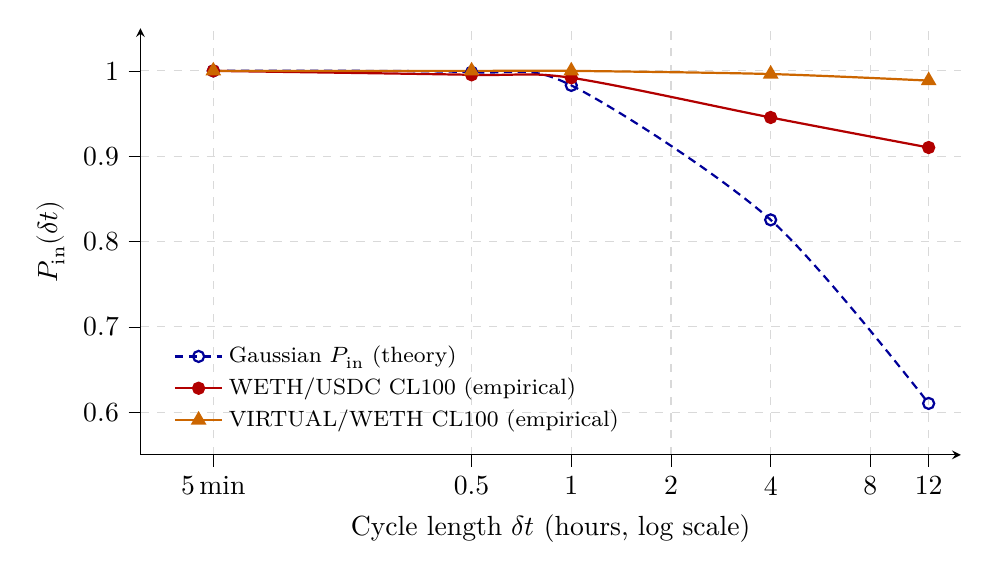
\begin{tikzpicture}
\begin{axis}[
  width=12cm, height=7cm,
  xlabel={Cycle length $\delta t$ (hours, log scale)},
  ylabel={$P_{\text{in}}(\delta t)$},
  xmode=log,
  log basis x=10,
  xmin=0.05, xmax=15,
  ymin=0.55, ymax=1.05,
  xtick={0.083,0.5,1,2,4,8,12},
  xticklabels={5\,min,0.5,1,2,4,8,12},
  ytick={0.6,0.7,0.8,0.9,1.0},
  legend pos=south west,
  legend cell align=left,
  legend style={font=\footnotesize,draw=none,fill=none},
  grid=major,
  grid style={dashed,gray!30},
  axis lines=left,
  tick align=outside,
  tick style={black},
  mark options={solid},
]
% Gaussian theoretical curve connecting computed points
\addplot[thick,blue!60!black,densely dashed,smooth,mark=o,mark size=2pt] coordinates {
  (0.083,1.0000)
  (0.5,0.9985)
  (1,0.9830)
  (4,0.8254)
  (12,0.6103)
};
\addlegendentry{Gaussian $P_{\text{in}}$ (theory)}

% WETH/USDC empirical points
\addplot[thick,smooth,mark=*,mark size=2pt,color=red!70!black] coordinates {
  (0.083,1.0000)
  (0.5,0.9954)
  (1,0.9919)
  (4,0.9454)
  (12,0.9102)
};
\addlegendentry{WETH/USDC CL100 (empirical)}

% VIRTUAL/WETH empirical points
\addplot[thick,smooth,mark=triangle*,mark size=2.5pt,color=orange!80!black] coordinates {
  (0.083,1.0000)
  (0.5,1.0000)
  (1,1.0000)
  (4,0.9963)
  (12,0.9886)
};
\addlegendentry{VIRTUAL/WETH CL100 (empirical)}
\end{axis}
\end{tikzpicture}
\caption{Empirical vs Gaussian $P_{\text{in}}$ for minimum-width positions ($w = 200$ ticks) on two Base mainnet CL100 pools. Sample size $N=1500$ starting times per pool. Short-cycle agreement is exact ($\delta t \leq 5$\,min: $P_{\text{in}} = 1$ under both models). Long-cycle departures run conservative: empirical $P_{\text{in}}$ exceeds Gaussian due to mean reversion, so Theorem~\ref{thm:parasitic} remains a valid upper bound.}
\label{fig:pinvalidation}
\end{figure}

For the tested pools at their current volatility, the range-exit scale~(\ref{eq:exitscale}) is
\[
\delta t^* \;\approx\; \frac{(a\eta)^2}{\sigma^2} \;=\; \frac{(100 \cdot 10^{-4})^2}{(8.93 \cdot 10^{-5})^2} \;\approx\; 1.25 \times 10^4\,\text{s} \;\approx\; 3.5\,\text{h}
\]
for a minimum-width position ($a = 100$ ticks on a CL100 pool). The Gaussian in-range probability formula is therefore a reliable tool at cycle times well below this scale, which covers the original Parasitic Liquidity attack's 2-second regime and the 10s-edge adversarial window discussed in~\S\ref{sec:composed}. At cycle times above $\delta t^*$, the per-position range filter of the CL gauge baseline itself already drives rewards to zero regardless of scoring function; the framework's distinguishing contribution operates in the short-cycle regime.

\subsection{Composed empirical suppression}\label{sec:composed}

Reference~\cite[\S5.3]{ryan2026c} reports parasitic extraction of $0.66\%$ of baseline under the combined minimum-width and warmup remediation against the pre-upgrade Aerodrome gauge (the ``unmitigated CL baseline'': a CL gauge with range-aware accumulator but no width, warmup, or concentration remediations). The three-correction framework (minimum width + warmup + concentration weighting) therefore bounds short-cycle parasitic extraction at no more than $0.66\%$ of the unmitigated CL baseline; the concentration factor provides additional width discrimination beyond the minimum-width floor, though at the measured $0.66\%$ level the marginal gain is small. Direct comparison with Aerodrome's post-upgrade step gate is deferred to~\S\ref{sec:threshold}.

% ---- 6. Calibration ----
\section{Calibration from operational data}\label{sec:calibration}

Parameter choices in the reference instance (Table~\ref{tab:reference}) are informed by an operational dataset of concentrated-liquidity rebalancing collected by the author over a 38-day pre-migration window (7~March to 13~April 2026). The window ends shortly before seven pools migrated to the post-upgrade Aerodrome gauge on and after 16~April (\S\ref{sec:composed}). The dataset contains $94{,}469$ rebalance events (after filtering numerical outliers from a raw $96{,}719$) across $48$ pools. Each event records the position's pre- and post-rebalance tick ranges, pre- and post-value in USD, geometric residual magnitude, and timestamp. A post-migration sub-window from those seven pools (16--21~April) is used in~\S\ref{sec:threshold} as a behavioural sanity check, not for calibration; the regime under the $10$\,s gate is materially different.

The dataset reflects active tight-range rebalancing under the unconstrained pre-upgrade gauge, within the active-management tail of~\cite{heimbach2022}. Under the proposed ramp, rational LPs lengthen cadence to raise $\bar f(\rho)$, so observed pre-constraint cadence overstates the cadence an equilibrium population would maintain; the calibration targets below are therefore upper bounds on drag.

\subsection{Observed width distribution}\label{sec:calwidth}

\begin{table}[H]
\centering
\begin{tabular}{@{}lr@{}}
\toprule
Quantile & Width (ticks) \\
\midrule
p25 & $67$ \\
Median & $200$ \\
p75 & $200$ \\
Mean & $176$ \\
\bottomrule
\end{tabular}
\caption{Position width distribution across $94{,}469$ rebalance events.}
\label{tab:width}
\end{table}

The median active position spans $200$ ticks, with the interquartile range running from $67$ to $200$ ticks. The distribution shifts mid-window. Events before 8~April concentrate around a $100$-tick median; from 8~April onwards positions widened for impermanent-loss and fee reasons independent of gauge mechanics, lifting the median to $200$ ticks. Both regimes sit in the non-capped regime of the reference concentration curve. With $w_{\text{ref}} = 1000 \times$ tickSpacing, the cap $c_{\max} = 100$ activates only at $w \leq w_{\text{ref}}/c_{\max}$, well below the observed p25 at typical active-LP tickSpacings, so the curve applies a smooth gradient across the observed distribution rather than clipping to the cap.

\subsection{Rebalance interval distribution}\label{sec:calinterval}

\begin{table}[H]
\centering
\begin{tabular}{@{}lrr@{}}
\toprule
Quantile & Seconds & Minutes \\
\midrule
p25 & $110$ & $1.8$ \\
Median & $368$ & $6.1$ \\
p75 & $958$ & $16.0$ \\
p95 & $4{,}682$ & $78.0$ \\
Mean & $1{,}201$ & $20.0$ \\
\bottomrule
\end{tabular}
\caption{Rebalance interval distribution across $94{,}267$ consecutive-rebalance pairs, grouped per wallet-pool (i.e.\ same operator in the same pool). Intervals capped at $1$~day; longer gaps excluded as operational downtime rather than LP behaviour.}
\label{tab:interval}
\end{table}

The median rebalance interval is $368$\,s (approximately $6$ minutes), with p25 at $110$\,s and p75 at $958$\,s. The lower tail reflects reactive rebalancing in volatile conditions; the upper tail reflects steady-state maintenance.

This distribution informs the warmup period $W$. Under Theorem~\ref{thm:legit}, the freshness drag for a legitimate LP is $W/(2\rho)$. The reference instance's $W = 20$\,s yields $2.7\%$ drag at the observed median $\rho = 368$\,s while suppressing $2$-second parasitic cycles by a factor of $2/(2 \cdot 20) = 0.05$. Shorter warmups ($W \approx 10$\,s) halve the drag at the median to $1.4\%$ with marginally weaker suppression of sub-second cycles. Longer warmups ($W \approx 60$\,s, proposed in~\cite[\S5.2]{ryan2026c}) produce $8.2\%$ drag at the observed median, still within a tolerable range. The $10$--$30$\,s range captures the defensible trade-off for pools dominated by active rebalancing. All drag figures are upper bounds, per the equilibrium-response argument in~\S\ref{sec:calibration}.

\subsection{Step-gate threshold impact on observed cadence}\label{sec:threshold}

Aerodrome's post-upgrade gauge~\cite{aerodrome2026} enforces a step-function freshness penalty with $\texttt{minStakeTimes}=10$\,s and $\texttt{penaltyRate}=10{,}000$ bps (full forfeit below threshold). A Foundry probe against the live CL100-WETH/VVV post-upgrade gauge (\texttt{test\_Post\-Upgrade\-Step\-Function}) measures zero rewards for $\delta t < 10$\,s and full rewards at $\delta t \geq 10$\,s, with identical per-second rate post-threshold. Figure~\ref{fig:freshness-compare} compares the step against the continuous ramp $\bar f(\delta t)$ from~(\ref{eq:fbar}). The step is stricter than the ramp below $10$\,s but leaves the interval $10 \leq \delta t < 2W = 40$\,s uncovered. An attacker cycling at $\delta t = 10.1$\,s defeats the production gate entirely, while the ramp applies $\bar f \approx 0.25$ suppression in the same regime.

\begin{figure}[H]
\centering
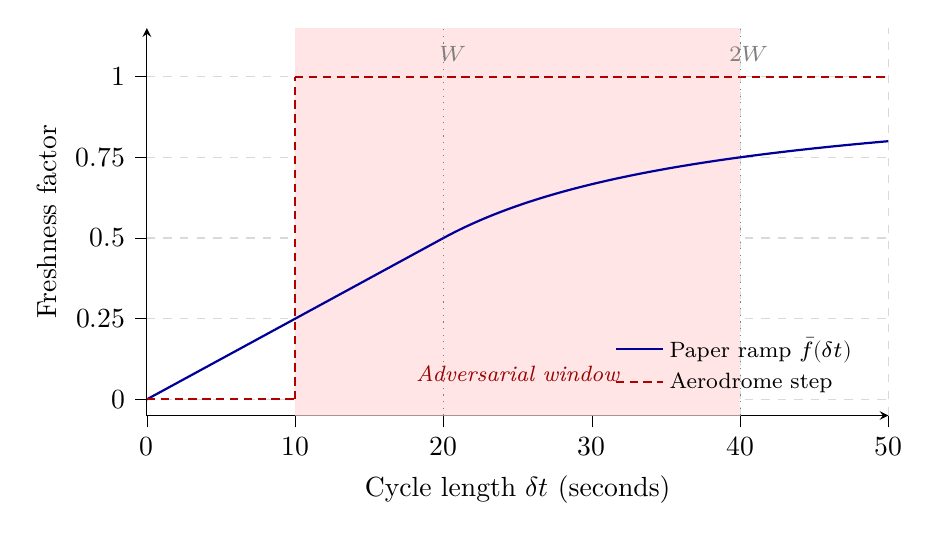
\begin{tikzpicture}
\begin{axis}[
  width=11cm, height=6.5cm,
  xlabel={Cycle length $\delta t$ (seconds)},
  ylabel={Freshness factor},
  xmin=0, xmax=50, ymin=-0.05, ymax=1.15,
  xtick={0,10,20,30,40,50},
  ytick={0,0.25,0.5,0.75,1.0},
  legend pos=south east,
  legend cell align=left,
  legend style={font=\footnotesize,draw=none,fill=none},
  grid=major,
  grid style={dashed,gray!30},
  axis lines=left,
  tick align=outside,
  tick style={black},
]
% Shaded adversarial window 10 <= dt < 40
\addplot[fill=red!10,draw=none,forget plot] coordinates {(10,-0.05) (40,-0.05) (40,1.15) (10,1.15)} \closedcycle;
\node[font=\footnotesize\itshape,text=red!60!black] at (axis cs:25,0.08) {Adversarial window};

% Paper ramp: bar f = dt/(2W) for dt <= W=20, then 1 - W/(2 dt) for dt > W
\addplot[thick,blue!60!black,domain=0:20,samples=50] {x/40};
\addplot[thick,blue!60!black,domain=20:50,samples=80,forget plot] {1 - 20/(2*x)};
\addlegendentry{Paper ramp $\bar f(\delta t)$}

% Aerodrome step: 0 for dt < 10, 1 for dt >= 10
\addplot[thick,red!70!black,densely dashed] coordinates {(0,0) (10,0)};
\addplot[thick,red!70!black,densely dashed,forget plot] coordinates {(10,0) (10,1)};
\addplot[thick,red!70!black,densely dashed,forget plot] coordinates {(10,1) (50,1)};
\addlegendentry{Aerodrome step}

% Mark W and 2W
\draw[gray,dotted] (axis cs:20,-0.05) -- (axis cs:20,1.15);
\node[font=\footnotesize,text=gray] at (axis cs:20.5,1.07) {$W$};
\draw[gray,dotted] (axis cs:40,-0.05) -- (axis cs:40,1.15);
\node[font=\footnotesize,text=gray] at (axis cs:40.5,1.07) {$2W$};
\end{axis}
\end{tikzpicture}
\caption{Freshness factor comparison: continuous ramp $\bar f(\delta t)$ (with $W = 20$\,s) vs Aerodrome's post-upgrade $10$\,s step gate. The ramp applies graded credit below $2W$ while the step binarises at a hard threshold. In the adversarial window $10 \leq \delta t < 2W = 40$\,s, the step pays in full and the ramp applies strict suppression; a $\delta t = 10.1$\,s parasitic cycle defeats the step entirely but incurs $\bar f \approx 0.25$ under the ramp.}
\label{fig:freshness-compare}
\end{figure}

Table~\ref{tab:threshold} shows the fraction of pre-upgrade rebalance intervals below each threshold $T$ and the reward treatment each band receives under (a) the continuous freshness ramp with $W = 20$\,s and (b) the $10$\,s step gate.

\begin{table}[H]
\centering
\begin{tabular}{@{}rrrll@{}}
\toprule
$T$ (s) & Count $< T$ & \% & Ramp credit & Step gate \\
\midrule
$5$   & $0$        & $0.00\%$ & --                & forfeit \\
$10$  & $3{,}825$  & $4.0\%$  & $\approx 23\%$    & forfeit \\
$15$  & $9{,}325$  & $9.7\%$  & $\approx 26\%$    & full reward \\
$20$  & $9{,}939$  & $10.3\%$ & $\approx 27\%$    & full reward \\
$30$  & $12{,}679$ & $13.1\%$ & $\approx 35\%$    & full reward \\
$60$  & $17{,}912$ & $18.6\%$ & $\approx 56\%$    & full reward \\
\bottomrule
\end{tabular}
\caption{Rebalance intervals below threshold $T$, over $96{,}517$ pre-upgrade consecutive-rebalance pairs (Mar 7 -- Apr 13, grouped per wallet and pool). ``Ramp avg credit'' reports the mean of $\bar f(\delta t)$ across intervals in each bucket (under $W = 20$\,s). ``Step gate'' reports Aerodrome's post-upgrade behaviour with $\texttt{penaltyRate} = 10{,}000$\,bps.}
\label{tab:threshold}
\end{table}

$4.0\%$ of intervals fall below the $10$\,s threshold ($12.7\%$ on WETH/USDC CL100 specifically), reflecting tight range-tracking in volatile conditions rather than gauge response since the dataset is pre-upgrade. The step forfeits these rewards in full; the ramp pays approximately $23\%$ at the mean sub-$10$\,s interval. In the $[10, 20)$\,s band ($6.3\%$ of intervals) the step pays in full while the ramp applies graded suppression. Under the step, an LP chooses between forfeiting short-cycle rewards and throttling rebalances to at least $10$\,s, the latter trading range-tracking precision for reward retention; the continuous ramp integrates the penalty over $[0, 2W]$ and imposes no such binary.

A post-migration sub-window provides a behavioural sanity check. Seven pools migrated to the post-upgrade gauge on or after 16~April (USDC/cbBTC, EURC/USDC, WETH/cbBTC, WETH/USDC at CL1; GIZA/USDC, TIBBIR/WETH, MEZO/MUSD at CL200); others stayed on the pre-upgrade gauge. Across the seven migrated pools over Apr 16--21 ($n = 666$ intervals), median cadence lengthened from $368$\,s to $1{,}919$\,s ($\approx 32$ minutes) and sub-$10$\,s intervals collapsed from $4.0\%$ to $0.2\%$. Median width held at $80$ ticks, consistent with the gate imposing a cadence floor rather than penalising concentration. Unmigrated pools show a separate, gate-independent widening driven by a pre-existing impermanent-loss adjustment and are not gate-response evidence. The sample is too thin for formal calibration, but the direction matches the trade-off above.

\subsection{Geometric residual distribution}\label{sec:calresidual}

\begin{table}[H]
\centering
\begin{tabular}{@{}lr@{}}
\toprule
Quantile & Leakage \\
\midrule
Median & $0.02\%$ \\
p75 & $4.79\%$ \\
p95 & $25.62\%$ \\
Mean & $4.71\%$ \\
\bottomrule
\end{tabular}
\caption{Absolute leakage (geometric residual magnitude relative to position value) per rebalance event.}
\label{tab:leakage}
\end{table}

Median single-event leakage is near zero. Same-range rebalances (Stage 2 of the mechanism in~\cite{ryan2026a}) produce no tick-mismatch residual and dominate the distribution. Tail leakage (p75 $\approx 5\%$, p95 $\approx 26\%$) comes from range-change events, with the tail thicker in the later wider-position portion of the window. Residual handling (whether or not a host protocol provides recycling infrastructure) is orthogonal to the scoring propositions but materially shapes the rebalance economics an LP faces in practice.

% ---- 7. Discussion ----
\section{Discussion}\label{sec:discussion}

\subsection{What the framework does not address}\label{sec:outofscope}

Several adjacent concerns fall outside the framework's scope:

\begin{itemize}[leftmargin=2em]
\item \textbf{Operational complexity for passive LPs.} Actively managing a concentrated liquidity position is costly in time and gas. The corrective framework rewards this activity but does not supply the infrastructure that makes it accessible to passive capital. Keeper networks, vault abstractions, and delegation patterns are complementary but out of scope.
\item \textbf{Geometric residuals from rebalancing.} Atomic rebalancing produces a residual token amount from the tick mismatch between consecutive ranges~\cite{ryan2026a}. Handling this residual is an implementation choice that affects capital efficiency but not the scoring framework.
\item \textbf{MEV protection for rebalance swaps.} Rebalances that involve a token swap are exposed to MEV; the gauge scoring does not address this. Protocol-level MEV protection (private mempools, commit-reveal, or post-swap slippage checks) is a distinct layer.
\item \textbf{Emission schedule and token economics.} The emission rate, decay curve, and allocation between LPs and token holders are governance variables unrelated to the distribution framework.
\item \textbf{Voting, bribing, and cross-pool allocation.} ve(3,3) and similar systems direct emissions across pools via voter weights. The corrective framework operates within a pool and does not modify these cross-pool mechanisms.
\end{itemize}

\subsection{Incentive compatibility}\label{sec:incentive}

The four factors of~(\ref{eq:score}) are monotone in the LP's choice variables (capital deployed, range width, rebalance frequency, range placement), so each of the protocol's desired behaviours (high-volume pool selection, concentration, rebalancing to stay in range, avoidance of purely nominal depth) weakly increases score and therefore weakly increases expected yield at fixed population scores. The alignment is monotone rather than equilibrium-optimal: intended behaviours dominate parasitic strategies within the scoring function without resolving the full multi-LP competitive equilibrium, which depends on population response and is out of scope. No LP trust or allow-listing is required; the score-monotone choices align with the intended behaviours structurally.

\subsection{Architectural framing in ve(3,3)}\label{sec:ve33}

The framework is designed for concentrated-liquidity gauges deployed in ve(3,3) protocols. In ve(3,3)~\cite{cronje2022}, emissions are a voter-directed subsidy. The inflation budget is allocated across pools by veNFT holders' votes; bribers pay voters to influence that direction; staked LPs within a pool receive emissions as payment for the liquidity voters wanted there. An unstaked LP earns swap fees directly from trades through their position, while a staked LP forfeits those fees to the pool's voters in exchange for the emission share. The separation between directed subsidy (to staked LPs) and organic revenue (to voters) is structural to the design.

In V2-era pools with fungible LP tokens, every staked position provides tradeable depth proportional to its token balance; staked liquidity and tradeable liquidity coincide. The Synthetix-style stake-proportional accumulator therefore distributes the subsidy along the criterion voters care about, and the literal mechanic (stake yields payment) matches the functional intent (real liquidity yields payment). In concentrated-liquidity deployments (Slipstream, PCS V3, and analogous CL AMMs), the equivalence breaks. A staked position can be narrow, held briefly, or out of range without providing meaningful depth. The parasitic vulnerability of~\cite{ryan2026c} is a composition accident of porting V2-era mechanics into a CL setting where staked liquidity and serviceable depth have diverged.

This divergence is specific to ve(3,3). Uniswap V3 fee accrual is self-pricing, since a position that captures fees has served swaps, and the rewarded and protocol-valued quantities coincide without additional mechanism. Ve(3,3) separates the two structurally. Staked LPs surrender fee income to voters and receive a share of a gauge-allocated emission budget computed by an independent formula. When that formula reduces to per-$L$ accrual on active-tick presence, a zero-volume position still collects its share, and the directed subsidy decouples from the outcome voters paid for. The corrective framework restores the coupling by making the within-pool formula track tradeable depth directly; voting, bribing, cross-pool allocation, and the fact of emissions accruing to staked LPs all remain unchanged.

Cronje's original design~\cite{cronje2022} placed no bound on voter-directed emission fraction per pool; production CL-era deployments (notably Aerodrome's per-gauge cap with cross-gauge redistribution) constrain voter direction as a defence against the extraction surface that opens when large flows meet a nominal-stake scoring formula. The corrective framework closes that surface at the per-LP measurement level.

Aerodrome's forthcoming Predictive Allocation~\cite{aerodrome2026pa}, scheduled for July 2026 with the Aero merger, replaces discrete weekly bribe voting with continuous real-time allocation in which token operators live-allocate emissions based on forward-looking forecasts of pool fee generation and are rewarded differentially by prediction accuracy. Predictive Allocation operates on cross-pool emission direction; the framework here operates on within-pool LP distribution. Predictive accuracy is easier when within-pool emissions flow to positions that actually serve volume, since pool-level fees are more stable when directed emissions attract real depth.

\subsection{Related deployed systems}\label{sec:relatedsystems}

Every in-production ve(3,3) CL gauge inspected for this paper uses the Synthetix \texttt{rewardPerToken} / \texttt{earned} pattern: Velodrome, Aerodrome (Slipstream), Ramses V2, Pharaoh, and Shadow operate on per-position liquidity via \texttt{rewardGrowthInside}; Thena V3.3 operates on fungible ERC20 wrappers of managed CL positions via the same Synthetix template. None weight by position width, time since deposit, or realised volume at the reward-math layer. Thena's V3.3 upgrade (May 2025) was announced with performance-framing marketing, but its active emission distribution runs through the Synthetix-style gauges rather than the Algebra farming layer, whose \texttt{factory.farmingAddress()} pointer shows zero event logs across sampled windows from mid-2025 onwards.

Algebra's stock eternal farming exposes an optional \texttt{minimalPositionWidth} parameter (\S\ref{sec:relatedwork}), used by QuickSwap on Polygon incentives. QuickSwap is not a ve(3,3) protocol: LPs earn swap fees directly and emissions are admin-allocated liquidity-mining rather than voter-directed subsidy, so the decoupling problem this paper targets does not arise in the same form there. QuickSwap's use of the parameter nonetheless demonstrates that minimum-width admission works in production on Algebra-powered CL. Slipstream-family gauges have no equivalent built-in, and no protocol is known to have forked one in; Thena's dormant farming layer means the parameter is not in effect for its production emissions either.

Merkl by Angle Labs~\cite{merkl2023} is the closest deployed analogue. It operates at the reward-distribution layer with off-chain computation and optimistic verification, while the corrective framework operates on-chain at the gauge scoring function with deterministic verification. Merkl's weights are also independently configurable per campaign without a structural argument that all three must be non-zero; Theorem~\ref{thm:mincomplete} provides that minimality here. Merkl has been used to supplement gauge emissions but not to replace the gauge formula, because ve(3,3)'s voter-fee flow and veNFT voting remain bound to the on-chain per-pool accumulator.

No deployed gauge inspected for this paper composes graded concentration, freshness, and an in-range factor at the LP-measurement layer, and none offers a structural argument for the joint necessity of the three analogous to Theorem~\ref{thm:mincomplete}.

% ---- 8. Conclusion ----
\section{Conclusion}\label{sec:conclusion}

Against a concentrated-liquidity gauge baseline, under the Gaussian log-price model and large-$N$ mean-field conditions, the corrective scoring function of~\S\ref{sec:framework} bounds parasitic extraction by the product of a freshness ratio and a concentration ratio (Theorem~\ref{thm:parasitic}) and imposes bounded drag on legitimate LPs (Theorem~\ref{thm:legit}). Structurally, the scoring function with all three corrections is the unique minimal member of the abstract product family closing all three parasitic pathways (Theorem~\ref{thm:mincomplete}); on CL gauge deployments the indicator is already supplied by the baseline accumulator, leaving $c$ and $f$ as the structurally novel corrections. Cross-chain fork tests against PancakeSwap V3, Thena FUSION, Ramses V2, and a reference implementation against live Aerodrome Slipstream (\S\ref{sec:empirical}), empirical validation of the in-range probability formula against live tick traces (\S\ref{sec:empirical-pin}), and calibration against an operational dataset of $94{,}469$ rebalance events (\S\ref{sec:calibration}) are consistent with the analysis and ground the parameter choices.

The algebraic change is local: the Synthetix accumulator's $L_i/\sum_j L_j$ becomes $S_i/\sum_j S_j$. With that substitution the measurement layer tracks tradeable depth contributed rather than nominal stake, and the quantity the gauge rewards becomes the quantity the protocol intended to reward.

% ---- References ----
\addcontentsline{toc}{section}{References}
\begin{thebibliography}{9}

\bibitem{ryan2026c}
Ryan, K.R.\ (2026c) `Parasitic Liquidity: Emission Extraction via Non-Functional Concentrated Liquidity Positions', \textit{SSRN Working Paper}. Available at: \url{https://doi.org/10.2139/ssrn.6510118}.

\bibitem{adams2021}
Adams, H., Zinsmeister, N., Salem, M., Keefer, R.\ and Robinson, D.\ (2021) `Uniswap v3 Core', \textit{Uniswap Labs Technical Whitepaper}. Available at: \url{https://uniswap.org/whitepaper-v3.pdf}.

\bibitem{synthetix2019}
Synthetix (2019) StakingRewards accumulator pattern (\texttt{rewardPerToken} / \texttt{earned}). Canonical Synthetix-deployed instance verified on-chain as \texttt{CurveRewards} at \texttt{0xDCB6A51eA3CA5d3Fd898Fd6564757c7aAeC3ca92} (MIT-licensed, Solidity 0.5.16, Synthetix: Old Deployer). Available at: \url{https://etherscan.io/address/0xDCB6A51eA3CA5d3Fd898Fd6564757c7aAeC3ca92\#code}.

\bibitem{cronje2022}
Cronje, A.\ (2022) `Solidly: preparation for launch', \textit{Medium}. Original post subsequently deleted; archived 29 April 2022 at \url{https://web.archive.org/web/20220429052133/https://andrecronje.medium.com/solidly-preparation-for-launch-8e653ce8a428}.

\bibitem{ryan2026a}
Ryan, K.R.\ (2026a) `The Geometric Siphon: Emergent Capital Reallocation in Concentrated Liquidity Portfolios', \textit{SSRN Working Paper}. Available at: \url{https://doi.org/10.2139/ssrn.6374838}.

\bibitem{ryan2026b}
Ryan, K.R.\ (2026b) `The Geometric Siphon II: Directional Properties', \textit{SSRN Working Paper}. Available at: \url{https://doi.org/10.2139/ssrn.6481498}.

\bibitem{heimbach2022}
Heimbach, L., Schertenleib, E.\ and Wattenhofer, R.\ (2022) `Risks and Returns of Uniswap V3 Liquidity Providers', in \textit{Proceedings of the 4th ACM Conference on Advances in Financial Technologies (AFT '22)}. Available at: \url{https://doi.org/10.1145/3558535.3559772}.

\bibitem{milionis2022b}
Milionis, J., Moallemi, C.C., Roughgarden, T.\ and Zhang, A.L.\ (2022) `Automated market making and loss-versus-rebalancing', \textit{arXiv preprint}, arXiv:2208.06046. Available at: \url{https://arxiv.org/abs/2208.06046}.

\bibitem{lloyd2023}
Lloyd, T., O'Broin, D.\ and Harrigan, M.\ (2023) `Emergent Outcomes of the veToken Model', \textit{arXiv preprint}, arXiv:2311.17589. Available at: \url{https://arxiv.org/abs/2311.17589}.

\bibitem{xiong2023}
Xiong, X., Wang, Z., Knottenbelt, W.\ and Huth, M.\ (2023) `Demystifying Just-in-Time (JIT) Liquidity Attacks on Uniswap V3', \textit{IACR Cryptology ePrint Archive}, Paper 2023/973. Available at: \url{https://eprint.iacr.org/2023/973}.

\bibitem{merkl2023}
Angle Labs (2023) `Merkl: Concentrated Liquidity Mechanisms', \textit{Merkl Documentation}. Available at: \url{https://docs.merkl.xyz/merkl-mechanisms/campaign-types/concentrated-liquidity-mechanisms}.

\bibitem{aerodrome2026}
Aerodrome Finance (2026) `Upgrades for a supersonic era', \textit{Medium}. Available at: \url{https://medium.com/@aerodromefi/upgrades-for-a-supersonic-era-1861487f40c6}.

\bibitem{aerodrome2026pa}
Aerodrome Finance (2026) `The economic case for Aero', \textit{aero.xyz}. Available at: \url{https://aero.xyz/articles/aero-economic-case/}.

\end{thebibliography}

% ---- Appendices ----
\clearpage
\appendix

\section{Empirical validation reproduction}\label{app:reproduction}

The empirical in-range probability validation in~\S\ref{sec:empirical-pin} was computed from live \texttt{Swap} event traces on Base mainnet.

\begin{enumerate}[leftmargin=2em]
\item Pull all \texttt{Swap} events from the target pool over a $24$-hour window (block range $[\text{head} - 43200, \text{head}]$ on Base, with $2$-second blocks). The Uniswap V3 swap event topic hash is \texttt{0xc42079f94a6350d7e6235f29174924f928cc2ac818eb64fed8004e115fbcca67}; the tick is the fifth $32$-byte word of the event data, decoded as a sign-extended \texttt{int24}.
\item Build a piecewise-constant tick function $\tau(b)$ keyed by block number.
\item Estimate realised volatility $\sigma$ by root-mean-square of standardised log-return increments: $\sigma = \sqrt{\mathbb{E}[(\Delta X / \sqrt{\Delta t})^2]}$ where $X = \tau \cdot \log(1.0001)$.
\item For each $(\delta t, w)$ pair, uniformly sample $N_s = 1500$ starting blocks from the trace (excluding a buffer equal to the maximum $\delta t$ from the trace end). For each sample $s$, compute the in-range fraction of $[s, s + \delta t / 2]$ (in blocks) for a position of half-width $w/2$ centred at $\tau(s)$.
\item Compare to the theoretical $P_{\text{in}}(\delta t; a, \sigma)$ from~(\ref{eq:pin}) by numerical integration ($400$ midpoint-rule nodes).
\end{enumerate}

The computation runs in under a minute per pool on a standard workstation with a single RPC endpoint.

\section{Fork test reproduction}\label{app:forktest}

The repository is at \url{https://github.com/g4nc0r/constructive-gauges}. The framework's fork-test results in Table~\ref{tab:forkmap} are reproduced by a minimal reference implementation of the scoring function. It implements equation~(\ref{eq:score}) with the parameter choices of Table~\ref{tab:reference} and a minimal Synthetix-style accumulator sufficient to reproduce the paper's numerical claims.

The suite runs against the Aerodrome Slipstream WETH/USDC CL100 pool on Base mainnet (\texttt{0xb2cc224c1c9feE385f8ad6a55b4d94E92359DC59}), with cross-chain replications on BSC and Arbitrum One. Reproduction from a clean checkout:

\begin{center}\begin{minipage}{0.85\textwidth}\begin{verbatim}
cd foundry
git submodule update --init --recursive

# Unit tests (no RPC needed)
forge test --match-contract MathTest -vv

# Base: Aerodrome Slipstream
BASE_RPC_URL=<your_base_rpc> forge test \
    --match-contract FrameworkForkTest -vv

# BSC: PancakeSwap V3 + Thena FUSION
BSC_RPC_URL=<your_bsc_rpc> forge test \
    --match-contract 'FrameworkBSCForkTest|FrameworkThenaForkTest' -vv

# Arbitrum: Ramses V2
ARB_RPC_URL=<your_arb_rpc> forge test \
    --match-contract FrameworkRamsesForkTest -vv
\end{verbatim}\end{minipage}\end{center}

Any working RPC endpoint is acceptable; the public endpoints \texttt{https://mainnet.base.org}, \texttt{https://bsc-dataseed.bnbchain.org}, and \texttt{https://arb1.arbitrum.io/rpc} are sufficient. Forge caches RPC responses, so repeat runs are fast.

Numerical values in Table~\ref{tab:forkmap} are single-run against live Base state and shift with pool state; qualitative claims hold deterministically.

\end{document}
